\chapter{谱不变量：构造}
\label{ch:spectral-construction}

为系统解释埃利亚什伯格的 $C^0$ 辛刚性结果，维泰博 (Vi92) 考察紧支哈密顿
微分同胚 $\phi$ 的图像，构造了 $\mathbb R^{2n}$ 上的一族辛不变量。他沿
$\mathbb R^{4n}=\mathbb R^{2n}\times\mathbb R^{2n}$ 的对角方向将此图像紧化到
$T^*S^{2n}$ 中，再把拉格朗日子流形 $\operatorname{graph}\phi\subset T^*S^{2n}$
的生成函数临界点理论以及任意闭光滑流形 $N$ 的余切丛 $T^*N$ 上的“稳定莫尔斯
理论”应用于它。当拉格朗日子流形 $L$ 带有生成函数时——例如 $L$ 与 $T^*N$ 的
零截面哈密顿同痕时——维泰博对每个上同调类 $a\in H^*(N)$ 都从给定生成函数
关联一个同调本质的临界值，并证明至少在相差归一化的意义下，它们只依赖于
拉格朗日子流形而不依赖于生成函数。

温斯坦观察到，作用量泛函是定义在给定哈密顿量 $H$ 的流把零截面送到
$\phi_H^1(o_N)$ 所对应道路空间上的生成函数。利用这一观察，笔者在 (Oh97b,
Oh99) 中发展了作用量泛函极小极大理论的弗洛尔理论方法，并构造出一族同样由
$H^*(N)$ 参数化的辛不变量，称为\emph{拉格朗日谱不变量}。此方法\emph{连同归一化}都是典范的，
并以透明的方式直接联系霍费尔几何与维泰博不变量。随后\personMilinkovic{}与笔者
证明，这族谱不变量在模掉归一化后确与维泰博不变量一致 (MiO95, Mi00)。

施瓦茨 (Schw00) 把类似方案用于\emph{辛非球面}的 $(M,\omega)$ 上的哈密顿不动点
弗洛尔理论；这里辛非球面意指
$c_1|_{\pi_2(M)}=\omega|_{\pi_2(M)}=0$。他由此得到一族由 $H^*(M)$ 参数化的
类似不变量。尤其是，他证明了谱不变量的重要最优三角不等式；在 (Oh97b, Oh99)
写作之时，上述拉格朗日谱不变量尚缺少这一结果。最近，\personMonzner{}、\personVichery{}与\personZapolsky{}也为拉格朗日谱不变量建立了相似的最优三角不等式 (MVZ12)。

在非正合辛流形上，作用量泛函不是单值的；弗洛尔同调理论须作为圆周值莫尔斯
理论，或作为可缩自由环路空间 $\mathcal L_0(M)$ 的覆盖空间
$\widetilde{\mathcal L}_0(M)$ 上的莫尔斯理论来发展。此时弗洛尔理论包含量子
效应，并本质地使用诺维科夫环。量子效应的出现，以及非有理辛流形上作用谱在
$\mathbb R$ 中的\emph{稠密性}，一直是研究\emph{哈密顿微分同胚族}时最严重的障碍。笔者继而在
(Oh02, Oh05c) 中，通过覆盖空间 $\widetilde{\mathcal L}_0(M)$ 上的链层弗洛尔
理论发展了一般的极小极大理论，并为每个给定的含时哈密顿量 $H$ 关联一族谱
不变量。此时这族不变量由量子上同调 $QH^*(M)$ 参数化，现在称为\emph{哈密顿谱不变量}。

\section{能量估计与霍费尔几何}
\label{sec:energy-estimates-hofer-geometry}

本节考察各种弗洛尔算子，以及它们如何改变复形 $CF^\lambda$ 的滤过层级。

固定哈密顿量 $H_\alpha,H_\beta$ 以及二者之间的同伦
$\mathcal H$。要强调的是，本节讨论中 $H_\alpha,H_\beta$ \emph{未必}非退化。选取相容殆复
结构的同伦 $j=\{J(\eta)\}_{0\leq\eta\leq1}$ 及截断函数
$\rho:\mathbb R\to[0,1]$，考虑相应弗洛尔方程
\begin{equation}
 \begin{cases}
 \partial u/\partial\tau+J^\rho
 (\partial u/\partial t-X_{H^\rho}(u))=0,\\
 u(-\infty)=z^-,\quad u(\infty)=z^+.
 \end{cases}
 \label{eq:21-floer-homotopy}
\end{equation}
下面的能量估计是联系作用量积分、弗洛尔连接流线的能量以及相应哈密顿量的霍费尔
范数的关键估计。它是命题~\ref{prop:20-energy-curvature-identity} 的特殊情形。这里给出一个
直接证明；在此特殊情形中它也颇具启发性，是引理 14.4.5 证明的一个变形。

\begin{proposition}
\label{prop:21-basic-energy-estimate}
设 $H_\alpha,H_\beta$ 是任意哈密顿量，不要求非退化；令
$\mathcal H=\{H^s\}_{0\leq s\leq1}$ 是二者之间的同伦。考虑对子
$(\mathcal H,j)$，并令 $\rho$ 是如前的任意截断函数。设 $u$ 满足
\eqref{eq:21-floer-homotopy}、$w^-\#u\sim w^+$（见 (19.4.16)），具有有限能量，
且对某些满足 $\tau_j^-\to-\infty,\tau_j^+\to\infty$ 的序列 $\tau_j^\pm$ 有
\[
 \lim_{j\to\infty}u(\tau_j^-)=z^-,\qquad
 \lim_{j\to\infty}u(\tau_j^+)=z^+.
\]
则\footnote{译者注：本命题只引入了端点哈密顿量 $H_\alpha,H_\beta$，原式却改用
$H,F$ 而未显式说明对应关系；译文照录原式记号。}
\begin{align}
 \mathcal A_F([z^+,w^+])-\mathcal A_H([z^-,w^-])
 &=-\int_{-\infty}^{\infty}\!\int_0^1
 \left\lVert\frac{\partial u}{\partial\tau}\right\rVert_{J^{\rho(\tau)}}^2
 \,dt\,d\tau \notag\\
 &\quad-\int_{-\infty}^{\infty}\rho'(\tau)\int_0^1
 \left.\frac{\partial H^s}{\partial s}\right|_{s=\rho(\tau)}
 (t,u(\tau,t))\,dt\,d\tau.
 \label{eq:21-action-energy-identity}
\end{align}
\end{proposition}

\begin{proof}
由同伦条件 $w^-\#u\sim w^+$，有
\[
 \int u^*\omega=\int(w^+)^*\omega-\int(w^-)^*\omega.
\]
更一般地，
\[
 \int_{w^-\#(u|_{-\infty<\tau'\leq\tau})}\omega
 =\int(w^-)^*\omega-\int_{-\infty}^{\tau}\!\int_0^1u^*\omega\,d\tau.
\]
为简化记号，以 $u(\tau)$ 表示环路 $t\mapsto u(\tau,t)$。若记
\[
 \widetilde u(\tau)=
 [u(\tau),w^-\#(u|_{-\infty<\tau'\leq\tau})],
\]
则
\[
 \mathcal A_F([z^+,w^+])-\mathcal A_H([z^-,w^-])
 =\int_{-\infty}^{\infty}\frac d{d\tau}
 \bigl(\mathcal A_{H^{\rho(\tau)}}(\widetilde u(\tau))\bigr)\,d\tau.
\]
计算得
\[
 \frac d{d\tau}\mathcal A_{H^{\rho(\tau)}}(\widetilde u(\tau))
 =d\mathcal A_{H^{\rho(\tau)}}(u(\tau))
 \left(\frac{\partial u}{\partial\tau}\right)
 -\int_0^1\frac{\partial H^{\rho(\tau)}}{\partial\tau}
 (\widetilde u(\tau,t))\,dt.
\]
这里 $d\mathcal A_{H^{\rho(\tau)}}(\widetilde u(\tau))$ 是固定 $\tau$ 后，哈密顿量
$H^{\rho(\tau)}=H^{\rho(\tau)}(t,x)$ 的作用量泛函在 $\widetilde u(\tau)$ 处的微分。
方程~\eqref{eq:21-floer-homotopy} 也是该含 $\tau$ 作用量泛函的负梯度流方程，故右端为
\[
 -\int_0^1\left\lVert\frac{\partial u}{\partial\tau}\right\rVert_{J_t^{\rho(\tau)}}^2dt
 -\rho'(\tau)\int_0^1
 \left.\frac{\partial H^s}{\partial s}\right|_{s=\rho(\tau)}
 (u(\tau,t))\,dt.
\]
在 $\tau\in\mathbb R$ 上积分即得~\eqref{eq:21-action-energy-identity}，证明完毕。
\end{proof}

现在从~\eqref{eq:21-action-energy-identity} 推出两条渐近轨道之间作用量差的各种结论。
先考察边界映射方程 (18.5.41)，即 $H_\alpha=H_\beta$ 且对所有
$s\in[0,1]$ 都有 $H^s\equiv H_\alpha$ 的情形。

\begin{corollary}
\label{cor:21-boundary-filtration}
对 (18.5.41) 满足 (19.4.16) 的任意有限能量解 $u$，有
\begin{equation}
 \mathcal A_H([z^+,w^+])-\mathcal A_H([z^-,w^-])
 \leq-\iint\left\lVert\frac{\partial u}{\partial\tau}\right\rVert_J^2\leq0.
 \label{eq:21-boundary-action-drop}
\end{equation}
特别地，当 $(H,J)$ 弗洛尔正则时，相应边界映射满足
\[
 \partial_{(H,J)}(CF_*^\lambda(H))\subset CF_*^\lambda(H),
\]
因而对任意 $\lambda\in\mathbb R$ 典范地限制为边界映射
\[
 \partial_{(H,J)}:(CF_*^\lambda(H),\partial_{(H,J)})
 \longrightarrow(CF_*^\lambda(H),\partial_{(H,J)}).
\]
\end{corollary}

接着考察链映射。下述结论立即来自~\eqref{eq:21-action-energy-identity}。

\begin{corollary}
\label{cor:21-continuation-energy}
设 $(\mathcal H,j;\rho)$ 与 $u$ 如命题~\ref{prop:21-basic-energy-estimate}，并设 $\rho$
单调。则
\begin{align}
 \mathcal A_F([z^+,w^+])-\mathcal A_H([z^-,w^-])
 &\leq-\iint\left\lVert\frac{\partial u}{\partial\tau}\right\rVert_{J^{\rho(\tau)}}^2
 +\int_0^1-\min_{x,s}\left(\frac{\partial H_t^s}{\partial s}\right)dt,
 \label{eq:21-continuation-action-bound}\\
 &\leq\int_0^1-\min_{x,s}\left(\frac{\partial H_t^s}{\partial s}\right)dt.
 \label{eq:21-continuation-action-bound-simple}
\end{align}
此外，\eqref{eq:21-continuation-action-bound} 可改写为能量上界
\footnote{译者注：原式第二项保留 $\tau\in(-\infty,\infty)$ 的积分，但被积式中既无
$\rho'(\tau)$ 也无 $\tau$ 依赖，并且末尾只排出 $dt$；此外，按
\eqref{eq:21-continuation-action-bound} 移项所得的作用量差应涉及
$\mathcal A_H([z^-,w^-])-\mathcal A_F([z^+,w^+])$，原式却把两组渐近端点对调。
译文均照录。}
\begin{equation}
 \iint\left\lVert\frac{\partial u}{\partial\tau}\right\rVert_{J^{\rho(\tau)}}^2
 \leq\mathcal A_H([z^+,w^+])-\mathcal A_F([z^-,w^-])
 +\int_{-\infty}^{\infty}\!\int_0^1
 -\min_{x,s}\left(\frac{\partial H_t^s}{\partial s}\right)dt.
 \label{eq:21-continuation-energy-bound}
\end{equation}
\end{corollary}

要强调的是，\emph{上述能量上界均不依赖于 $u$，也不依赖于 $j,\rho,J$ 的选取；它们只
依赖于同伦 $\mathcal H$ 本身}及 $u$ 的渐近条件。受~\eqref{eq:21-continuation-action-bound-simple}
启发，引入如下定义。

\begin{definition}
\label{def:21-homotopy-variation}
设 $\mathcal H=\{H(s)\}_{0\leq s\leq1}$ 是哈密顿量的同伦。定义其变分的\emph{负部}与\emph{正部}为
\[
 E^-(\mathcal H):=\int_0^1-\min_{x,s}\left(\frac{\partial H_t^s}{\partial s}\right)dt,
 \qquad
 E^+(\mathcal H):=\int_0^1\max_{x,s}\left(\frac{\partial H_t^s}{\partial s}\right)dt,
\]
并定义\emph{总变分}
\[
 E(\mathcal H)=E^-(\mathcal H)+E^+(\mathcal H).
\]
\end{definition}

若以 $\mathcal H^{-1}$ 表示 $\mathcal H$ 的时间反演，即
\[
 \mathcal H^{-1}:s\in[0,1]\longmapsto H^{1-s},
\]
则
\[
 E^\pm(\mathcal H^{-1})=E^\mp(\mathcal H),\qquad
 E(\mathcal H^{-1})=E(\mathcal H).
\]
把这些定义用于端点 $H(0),H(1)$ 非退化的对子 $(\mathcal H,j)$，当 $\rho$ 单调时，
先验能量估计~\eqref{eq:21-continuation-action-bound-simple} 写成
\[
 \iint\left\lVert\frac{\partial u}{\partial\tau}\right\rVert_{J^{\rho(\tau)}}^2
 \leq-\mathcal A_F(u(\infty))+\mathcal A_H(u(-\infty))+E^-(\mathcal H).
\]
这里回忆：哈密顿量非退化时，命题 18.5.3 保证任意有限能量解在
$\tau\to\pm\infty$ 时都有良定义的渐近极限。

记相应滤过同调为 $HF_*^\lambda(H,J)$，称之为滤过弗洛尔同调群。

\begin{corollary}
\label{cor:21-filtered-continuation-map}
设 $(H^0,J^0)$、$(H^1,J^1)$ 弗洛尔正则，$(\mathcal H,j)$ 是连接二者的弗洛尔
正则道路，且 $\rho$ 如前。则链映射 $h_{(\mathcal H,j;\rho)}$ 满足
\[
 h_{(\mathcal H,j;\rho)}(CF_*^\lambda(H^0))
 \subset CF_*^{\lambda+E^-(\mathcal H)}(H^1),
\]
因而典范地限制为链映射
\[
 h_{(\mathcal H,j;\rho)}:
 (CF_*^\lambda(H^0),\partial_{(H^0,J^0)})\longrightarrow
 (CF_*^{\lambda+E^-(\mathcal H)}(H^1),\partial_{(H^1,J^1)}).
\]
\end{corollary}

下面单独指出推论~\ref{cor:21-continuation-energy}、\ref{cor:21-filtered-continuation-map}
的一个特殊情形；稍后构造谱不变量 $\rho(H;a)$ 时会用到它。回忆在 12.5.2 节构造
余切丛上拉格朗日子流形的谱不变量时，也曾使用同一结果。

\begin{corollary}
\label{cor:21-change-almost-complex-structure}
给定 $H$。考虑两个 $J^0,J^1$、一个\termElongationFunction{}~$\rho$，以及连接
$(H,J^0)$ 与 $(H,J^1)$ 且满足 $\mathcal H\equiv H$ 的同伦 $(\mathcal H,j)$。
对 (18.5.42) 满足 (19.4.16) 的任意有限能量解 $u$，有
\begin{equation}
 \mathcal A_H([z^+,w^+])-\mathcal A_H([z^-,w^-])
 \leq-\iint\left\lVert\frac{\partial u}{\partial\tau}\right\rVert_{J^{\rho(\tau)}}^2
 \leq0.
 \label{eq:21-fixed-hamiltonian-energy}
\end{equation}
特别地，若 $H$ 非退化，$J^0,J^1$ 是 $H$-正则的且 $(H,j)$ 通有，则相应链映射满足
\[
 h_{(H,j;\rho)}(CF_*^\lambda(H))\subset CF_*^\lambda(H),
\]
并典范地限制为链映射
\[
 h^\lambda_{(H,j;\rho)}:
 (CF_*^\lambda(H),\partial_{(H,J^0)})\longrightarrow
 (CF_*^\lambda(H),\partial_{(H,J^1)}),
\]
且对任意 $\lambda\in\mathbb R$ 都在同调上诱导同构。
\end{corollary}

\begin{proof}
只须证明 $h^\lambda_{(H,j;\rho)}$ 在同调上诱导同构。选取从 $J^1$ 连接到 $J^0$
且弗洛尔正则的同伦 $j'$ 及截断函数 $\rho$。
\footnote{译者注：原文此处选取 $j'$，却写“使 $(H,j)$ \personFloer{}正则”；译文按语境
改为 $j'$。}
同伦 $j\#j'$ 从 $J^0$ 连接到
$J^0$。把它形变到常同伦 $j_{\mathrm{const}}\equiv J^0$，并以 $\overline j$ 表示
从 $j_{\mathrm{const}}$ 连接到 $j\#j'$ 的同伦的同伦。由
\eqref{eq:21-fixed-hamiltonian-energy}，$(H,\overline j)$ 给出
$h_{(H,j_{\mathrm{const}};\rho)}$ 与 $h_{(H,j)\#(\rho;R)(H,j')}$ 之间的链同伦。
因 $j_{\mathrm{const}}\equiv J^0$，$(H^\rho,j_{\mathrm{const}}^\rho)$ 是常同伦
$(H,J^0)$；由 $(H,J^0)$ \emph{作为族}的弗洛尔正则性，
$h_{(H,j_{\mathrm{const}};\rho)}=\mathrm{id}$。另一方面，取充分大的 $R>0$，粘合恒等式为
\[
 h_{(H,j)\#(\rho;R)(H,j')}=h_{(H,j';\rho)}\circ h_{(H,j;\rho)}.
\]
故在 $HF_*^\lambda(H,J^0)$ 上该复合等于恒等。交换 $j,j'$ 同理证明另一复合在
$HF_*^\lambda(H,J^1)$ 上等于恒等。
\end{proof}

\begin{remark}
\label{rem:21-filtered-local-system}
此推论也可表述为：对每个给定哈密顿量 $H$ 和层级 $\lambda\in\mathbb R$，赋值
$J\in\mathcal J_\omega\mapsto HF_*^\lambda(H,J)$ 在 $\mathcal J_\omega$ 上定义一个
局部系统。
\end{remark}

现在把上述滤过变化同哈密顿道路的霍费尔范数联系起来。在霍费尔几何中定义
\[
 E^-(H)=\int_0^1-\min_xH_t\,dt,\qquad
 E^+(H)=\int_0^1\max_xH_t\,dt,
\]
以及
\[
 \lVert H\rVert=E^+(H)+E^-(H)
 =\int_0^1(\max_xH_t-\min_xH_t)\,dt.
\]
例如参见 (Po01)、(Oh05d)。当 $\mathcal H$ 是连接 $H_1,H_2$ 的线性同伦
\[
 \mathcal H^{\mathrm{lin}}:s\longmapsto(1-s)H_1+sH_2,
\]
$E^\pm(\mathcal H^{\mathrm{lin}})$ 与 $E(\mathcal H^{\mathrm{lin}})$ 分别成为
$E^\pm(H_2-H_1)$ 与 $\lVert H_2-H_1\rVert$。事实上，$E^\pm(H)$ 或 $E(H)$ 可视为
\emph{线性道路} $s\mapsto sH$ 在定义~\ref{def:21-homotopy-variation} 意义下的变分。不过，
当 $H$ 非自治时，这条线性道路从 $\operatorname{Ham}(M,\omega)$ 本身的几何来看
并没有多少内蕴意义。

\begin{remark}
\label{rem:21-hofer-norm-universal-cover}
即使 $H\sim F$，也可能
\[
 \lVert H\rVert\neq\lVert F\rVert.
\]
因此 $H\mapsto\lVert H\rVert$ 不能下降到万有覆盖
$\pi:\widetilde{\operatorname{Ham}}(M,\omega)\to\operatorname{Ham}(M,\omega)$。
定义 $h\in\widetilde{\operatorname{Ham}}(M,\omega)$ 的不变量的一种标准方式是取下确界
\begin{equation}
 \lVert h\rVert:=\inf_{[H]=h}\lVert H\rVert
 =\inf_{[H]=h}\operatorname{leng}(\phi_H).
 \label{eq:21-hofer-norm-cover}
\end{equation}
函数 $h\mapsto\lVert h\rVert\in\mathbb R_+$ 先验地\emph{未必}关于
$\widetilde{\operatorname{Ham}}(M,\omega)$ 上的自然拓扑连续。
\end{remark}

对端点固定为 $H(0)=H^0,H(1)=H^1$ 的所有 $\mathcal H$，取 $E(\mathcal H)$ 的下确界，
得到
\[
 \inf_{\mathcal H}\{E(\mathcal H)\mid H(0)=H^0,H(1)=H^1\}
 \leq\lVert H^1-H^0\rVert,
\]
一般而言这是严格不等式。左端量的几何意义恰是定义 4.3.3 所引入的哈密顿纤维化
之大小；其渐近和乐为
\[
 ([\phi_{H^0}],[\phi_{H^1}]).
\]

\stfhIndex{I081}{Fuluoerliantonglunyingshe}{弗洛尔链同伦映射（Floer chain homotopy map）}
下面研究弗洛尔链同伦映射。考虑非退化哈密顿量 $H$、弗洛尔正则对子 $(H,J)$，
以及连接这些对子且弗洛尔正则的同伦 $(\mathcal H,j)$。还考虑同伦的同伦
$(\overline{\mathcal H},\overline j)$，其中
$\overline{\mathcal H}=\{\mathcal H_\kappa\}_{0\leq\kappa\leq1}$、
$\overline j=\{j_\kappa\}_{0\leq\kappa\leq1}$，并记诱导的链同伦映射为
$\Upsilon_{\overline{\mathcal H}}=H(\overline{\mathcal H},\overline j;\rho)$。
下述命题描述弗洛尔链 $\alpha$ 的层级在各种弗洛尔算子下如何变化。

\begin{proposition}
\label{prop:21-floer-operator-levels}
设 $\rho$ 是（正向）单调截断函数。\footnote{译者注：命题开头假设 $\rho$ 为正向单调截断函数，而第 (2) 项又声称
“对任意 $\rho$”；两处照录。}
\begin{enumerate}[label=(\arabic*)]
 \item 对任意弗洛尔链 $\alpha$，
 $\lambda_H(\partial_{(H,J)}\alpha)<\lambda_H(\alpha)$。
 \item 对任意 $\rho$，
 $\lambda_{H^1}(h_{(\mathcal H,j;\rho)}(\alpha))
 \leq\lambda_{H^0}(\alpha)+E^-(\mathcal H)$。
 \item $\lambda_{H^1}(\Upsilon_{\overline{\mathcal H}}(\alpha))
 \leq\lambda_{H^0}(\alpha)+\max_{\kappa\in[0,1]}E^-(\mathcal H_\kappa)$。
\end{enumerate}
\end{proposition}

\begin{proof}
前两项立即来自推论~\ref{cor:21-continuation-energy}。证明第 (3) 项时，令
$[z',w']\in\operatorname{Crit}\mathcal A_{H^1}$ 是该链的峰。按
$\Upsilon_{\overline{\mathcal H}}(\alpha)$ 的定义，存在 $\alpha$ 的生成元
$[z,w]\in\operatorname{Crit}\mathcal A_{H^0}$ 与某个 $\kappa\in(0,1)$，使方程
\begin{equation}
 \frac{\partial u}{\partial\tau}
 +J^{\kappa,\rho}\left(\frac{\partial u}{\partial t}-X_{H^{\kappa,\rho}}(u)\right)=0
 \label{eq:21-chain-homotopy-equation}
\end{equation}
在渐近条件
\[
 u(-\infty)=[z,w],\qquad u(\infty)=[z',w']
\]
下有解。由~\eqref{eq:21-continuation-action-bound-simple}，
\begin{equation}
 \mathcal A_{H^1}([z',w'])
 \leq\mathcal A_{H^0}([z,w])+E^-(\mathcal H_\kappa).
 \label{eq:21-chain-homotopy-action}
\end{equation}
因 $[z',w']$ 是峰，对对子 $(\mathcal H_\kappa,j_\kappa)$ 使用同样论证与层级定义即得
\[
 \lambda_{H^1}(\Upsilon_{\overline{\mathcal H}}(\alpha))
 \leq\lambda_{H^0}(\alpha)+E^-(\mathcal H_\kappa).
\]
对 $\kappa\in(0,1)$ 取上确界即证。
\footnote{译者注：原文在此把此前定义的链同伦映射
$H_{\overline{\mathcal H}}$ 称为 ``chain map''；译文按其实际角色写作
$\Upsilon_{\overline{\mathcal H}}$。}
\end{proof}

记
\[
 E^-(\overline{\mathcal H}):=
 \max_{\kappa\in[0,1]}E^-(\mathcal H_\kappa).
\]
命题~\ref{prop:21-floer-operator-levels}(3) 给出：

\begin{corollary}
\label{cor:21-chain-homotopy-filtration}
设 $(H^0,J^0)$ 与 $(H^1,J^1)$ 是两个弗洛尔正则对子，并考虑同伦的通有同伦
$(\overline{\mathcal H},\overline j)$，其中每个 $\mathcal H_\kappa$ 都连接二者。
则诱导的链同伦映射满足
\[
 \Upsilon_{\overline{\mathcal H}}(CF^\lambda(H^0))
 \subset CF^{\lambda+E^-(\overline{\mathcal H})}(H^1).
\]
\end{corollary}

最后把滤过变化同扰动柯西--黎曼方程所伴随的 $\epsilon$-正则性型不变量联系
起来。先注意，$\mathcal J=\{J_t\}_{0\leq t\leq1}$ 是紧族，因为 $[0,1]$ 紧。
给定非退化哈密顿函数 $H$，对每个 $H$-正则的 $J$ 考虑
\[
 \frac{\partial u}{\partial\tau}
 +J\left(\frac{\partial u}{\partial t}-X_H(u)\right)=0.
\]
若解 $u$ 与 $\tau$ 无关，称它是\emph{定常}的。定义
\[
 A_{(H,J)}:=\inf\left\{\int\left\lVert\frac{\partial u}{\partial\tau}\right\rVert_J^2
 \ \middle|\ u\text{ 满足 (18.5.41) 且\termNonStationary{}}\right\}>0
\]
及
\[
 A^\mu_{(H,J)}:=\inf\left\{\int\left\lVert\frac{\partial u}{\partial\tau}\right\rVert_J^2
 \ \middle|\ u\text{ 满足 (18.5.41) 且 }\mu_H(u)=1\right\}.
\]
显然 $A^\mu_{(H,J)}\geq A_{(H,J)}>0$。于是命题~\ref{prop:21-floer-operator-levels}(1)
可加强为：对任意弗洛尔链 $\alpha$，
\begin{equation}
 \lambda_H(\partial_{(H,J)}\alpha)
 \leq\lambda_H(\alpha)-A^\mu_{(H,J)}.
 \label{eq:21-boundary-uniform-drop}
\end{equation}

\section{\texorpdfstring{哈密顿量 $H$ 的边界深度}{哈密顿量 H 的边界深度}}
\label{sec:hamiltonian-boundary-depth}

在着手构造谱不变量 $\rho(H;a)$ 之前，先定义哈密顿量 $H$ 所伴随的一个更为朴素的
\stfhIndex{I043}{00-beta-h}{$\beta(H)$}
不变量，即\termBoundaryDepth{}~$\beta(H)$；它是 13.8 节定义 13.8.5 的特殊情形。
我们将证明，$\beta(H)$ 是滤过链复形 $CF_*(H)$ 的同构型不变量。

\begin{definition}[边界深度]
\label{def:21-hamiltonian-boundary-depth}
设 $H$ 是给定的非退化哈密顿量，并设 $(H,J)$ 弗洛尔正则。对相应弗洛尔复形
$(CF_*(H,J),\partial_{(H,J)})$，定义
$\beta(H,J):=\beta(\partial_{(H,J)})$，即
\[
 \beta(H,J)=\inf\bigl\{\beta\in\mathbb R\mid
 \forall\lambda\in\mathbb R,\space
 CF_*^\lambda(H,J)\cap\partial CF_*(H,J)
 \subset\partial(CF_*^{\lambda+\beta}(H,J))\bigr\}.
\]
\end{definition}

下述引理立即来自推论~\ref{cor:21-change-almost-complex-structure}。

\begin{lemma}
\label{lem:21-boundary-depth-independent-j}
设 $H$ 非退化，且 $(H,J^0)$、$(H,J^1)$ 均弗洛尔正则，则
\[
 \beta(H,J^0)=\beta(H,J^1).
\]
\end{lemma}

\begin{proof}
证明 $\beta(H,J^0)\leq\beta(H,J^1)$，反向同理。只须证明：若 $\beta\geq0$ 满足
\[
 CF_*^\lambda(H,J^0)\cap\partial CF_*(H,J^0)
 \subset\partial(CF_*^{\lambda+\beta}(H,J^0)),
\]
则对任意 $\epsilon>0$，
\begin{equation}
 CF_*^\lambda(H,J^1)\cap\partial CF_*(H,J^1)
 \subset\partial(CF_*^{\lambda+\beta+\epsilon}(H,J^1)).
 \label{eq:21-boundary-depth-transfer}
\end{equation}
选取从 $J^0$ 到 $J^1$、相对于 $H$ 正则的道路 $j$，记相应链映射为
$h_{(H,j)}:CF_*(H,J^0)\to CF_*(H,J^1)$。由推论
\ref{cor:21-change-almost-complex-structure}，对每个
$\lambda\in\mathbb R\setminus\operatorname{Spec}(H)$，它限制为链同构
\footnote{译者注：原文称 $h_{(H,j)}^\lambda$ 为链同构；但所引推论
\ref{cor:21-change-almost-complex-structure} 只断言它是链映射且在同调上诱导同构。
译文照录原断言。}
\[
 h_{(H,j)}^\lambda:CF_*^\lambda(H,J^0)\longrightarrow CF_*^\lambda(H,J^1),
\]
且
\[
 h_{(H,j)}^\lambda\circ\partial_{(H,J^0)}
 =\partial_{(H,J^1)}\circ h_{(H,j)}^\lambda.
\]
因此，若 $\lambda+\beta\notin\operatorname{Spec}(H)$，则
\eqref{eq:21-boundary-depth-transfer} 甚至可取 $\epsilon=0$；否则可取任意满足
$\lambda+\beta+\epsilon\notin\operatorname{Spec}(H)$ 的 $\epsilon>0$。因
$\mathbb R\setminus\operatorname{Spec}(H)$ 在 $\mathbb R$ 中稠密，$\epsilon$ 可任意小。
交换 $J^0,J^1$ 即完成证明。
\end{proof}

据此，今后简记 $\beta(H)=\beta(H,J)$，其中 $J$ 是使 $(H,J)$ 弗洛尔正则的任一
\stfhIndex{I190}{Eshe}{厄舍（Usher）}
选择。厄舍在 (Ush11) 中证明了边界深度的下列基本性质。（与第 (2) 项相似的结论
见 (Oh09a) 的命题 8.8。）

\begin{theorem}[厄舍]
\label{thm:21-boundary-depth-properties}
边界深度 $\beta$ 满足：
\begin{enumerate}[label=(\arabic*)]
 \item 若 $H,K$ 是两个非退化哈密顿量，则
 \[
  |\beta(H)-\beta(K)|\leq\lVert H-K\rVert.
 \]
 特别地，$\beta$ 关于 $L^{(1,\infty)}$ 拓扑利普希茨连续，因而在该拓扑下连续
 延拓为非负函数。
 \item $\beta(H)\leq\lVert H\rVert$。
 \item 若非退化哈密顿量 $H,K$ 满足 $H\sim K$，则 $\beta(H)=\beta(K)$。
\end{enumerate}
\end{theorem}

\begin{proof}
考虑线性同伦 $\mathcal H^{\mathrm{lin}}:s\mapsto(1-s)H+sK$。可为之选取适当的
$\mathcal J$，使 $(\mathcal H^{\mathrm{lin}},\mathcal J)$ 弗洛尔正则。仍然只须证明
\begin{equation}
 \beta(H)\leq\beta(K)+\lVert H-K\rVert
 \label{eq:21-boundary-depth-lipschitz}
\end{equation}
及交换 $H,K$ 后的版本。沿用引理~\ref{lem:21-boundary-depth-independent-j} 的论证，
这次对 $\mathcal H=\mathcal H^{\mathrm{lin}}$ 使用推论
\ref{cor:21-filtered-continuation-map}，即得~\eqref{eq:21-boundary-depth-lipschitz}，从而
证明第 (1) 项。令 $K\to0$ 得第 (2) 项。最后，引理
\ref{lem:21-boundary-depth-independent-j} 的同一证明适用于第 (3) 项；此时使用
21.6.2 节的推论~\ref{cor:21-optimal-continuation-filtration}。
\footnote{译者注：原文写“21.6.2 节的推论 21.1.5”，但推论 21.1.5 不在该节；
按论证所需的保滤过结论改引推论 21.6.5。}
\end{proof}

正如厄舍 (Ush11) 所指出的，该定理说明 $\beta(H)$ 是滤过链复形 $CF_*(H,J)$ 的
同构型不变量。边界深度与下一节将构造的谱不变量 $\rho(H;a)$ 有一点有趣的区别：
它确实是复形 $CF_*(H,J)$ 的不变量，却不像谱不变量那样出自同调层面的理由。
\footnote{译者注：原文此处写作“将在下一章构造”，但谱不变量紧接着在本章
21.3 节构造；译文按实际结构改作“下一节”。}
关于边界深度在辛拓扑和哈密顿动力系统各类问题中的有趣应用，参见 (Ush11)、
(Ush12)、(Ush13)。

\section{谱不变量的定义及其公理}
\label{sec:spectral-invariants-definition-axioms}

本节\emph{不}假设 $H$ 已归一化，但对任意给定哈密顿量，以 $\underline H$ 表示其归一化：
\begin{equation}
 \underline H(t,x)=H(t,x)-\frac1{\operatorname{vol}_\omega(M)}
 \int_MH(t,x)\,\mu_\omega.
 \label{eq:21-hamiltonian-normalization}
\end{equation}

\subsection{谱不变量的定义}

对每个给定的齐次量子上同调类 $a\in QH^*(M)$，记
$a^\flat=a_H^\flat\in HF_*(H,J)$ 为其在同构 $\Phi_H$ 下的像。记
\[
 i^\lambda:HF_*^\lambda(H,J)\longrightarrow HF_*(H,J)
\]
为由典范包含诱导的同态。

\begin{definition}
\label{def:21-spectral-invariant}
设 $H$ 是非退化的一周期哈密顿量，$J$ 是 $H$-正则的。对任意给定的
$0\neq a\in QH^*(M)$，考虑对子 $(H,J)$ 的弗洛尔闭链
$\alpha\in\ker\partial_{(H,J)}\subset CF_*(H)$，使其代表 $a^\flat$。定义
\[
 \rho((H,J);a):=\inf_{\alpha;\,[\alpha]=a^\flat}\lambda_H(\alpha),
\]
等价地，
\[
 \rho((H,J);a):=
 \inf\{\lambda\in\mathbb R\mid a^\flat\in\operatorname{Im}i^\lambda
 \subset HF_*(H,J)\}.
\]
\end{definition}

下面是关于谱数非平凡性的基本定理。厄舍 (Ush08) 在弗洛尔同调的抽象表述中给出
了 $\rho((H,J);a)$ 有限性的纯代数证明。这里的证明改编自 (Oh05c)、(Oh06a) 与
(Ush08) 中相应结论的证明。

\begin{theorem}
\label{thm:21-spectral-invariant-finite-independent}
设 $H$ 非退化，$0\neq a\in QH^*(M)$。
\begin{enumerate}[label=(\arabic*)]
 \item 对任意 $H$-正则的 $J$，$\rho((H,J);a)>-\infty$。
 \item $\rho((H,J);a)$ 的定义与 $H$-正则的 $J$ 的选取无关；公共值记为
 $\rho(H;a)$。
\end{enumerate}
\end{theorem}

\begin{proof}
由定理~\ref{thm:21-boundary-depth-properties}(2) 及边界深度的定义，
\begin{equation}
 \partial(CF_*(H,J))\cap CF_*^\lambda(H,J)
 \subset\partial(CF_*^{\lambda+\lVert H\rVert}(H,J)).
 \label{eq:21-boundary-depth-control}
\end{equation}
以下命题是弗洛尔理论极小极大法中的重要成分，对应于经典临界点理论中“极小极大
集合”的关键\emph{\termLinkingProperty{}}（这种观点例如见 (Bn82)）。

\begin{proposition}
\label{prop:21-floer-minimax-lower-bound}
设 $\alpha$ 是 $CF_*(H,J)$ 中的 $\partial$-闭链，且其同调类
$[\alpha]\neq0$，其中 $\partial=\partial_{(H,J)}$。则
\begin{equation}
 \inf_{\beta\in CF_*(H,J)}\{\lambda_H(\alpha-\partial\beta)\}>-\infty.
 \label{eq:21-minimax-finite}
\end{equation}
\end{proposition}

\begin{proof}
反设存在 $\beta_j\in CF_*(H,J)$ 使
$\lambda_H(\alpha-\partial\beta_j)\to-\infty$。记
\begin{equation}
 \lambda_j=\lambda_H(\alpha-\partial\beta_j).
 \label{eq:21-lambda-sequence}
\end{equation}
取子列后可设 $\lambda_j>\lambda_{j+1}$。归纳构造序列 $\beta'_k$，使
\begin{align}
 \lambda_H(\alpha-\partial\beta'_k)&\leq\lambda_k,
 \label{eq:21-beta-prime-cycle-bound}\\
 \lambda_H(\beta'_{k+1}-\beta'_k)&\leq\lambda_k+\lVert H\rVert.
 \label{eq:21-beta-prime-cauchy-bound}
\end{align}
一旦构成，令 $\alpha_N=\alpha-\partial\beta'_N$。由
\eqref{eq:21-beta-prime-cycle-bound} 与 $\lambda_j\to-\infty$，有
$[\alpha_N]=[\alpha]$ 且 $\alpha_N$ 在 $\lambda_H$ 非阿基米德拓扑中趋于 $0$。
另一方面，\eqref{eq:21-beta-prime-cauchy-bound} 表明 $\beta'_j$ 在
$CF_*(H,J)$ 的 $\lambda_H$ 非阿基米德拓扑中收敛。记极限为 $\beta'_\infty$。
因 $\partial$ 关于该拓扑连续，$\partial\beta'_N\to\partial\beta'_\infty$，故
$\alpha=\partial\beta'_\infty$，与 $[\alpha]\neq0$ 矛盾。

余下只须构造 $\beta'_j$。令 $\beta'_1=\beta_1$。我们将证明：在 $\beta'_k$ 已满足
\eqref{eq:21-beta-prime-cycle-bound} 的假设下，下述构造给出的 $\beta'_{k+1}$
满足把 $k$ 换成 $k+1$ 后的 \eqref{eq:21-beta-prime-cycle-bound}。由于
\[
 \lambda_H(\alpha-\partial\beta'_k)\leq\lambda_k,
 \quad \lambda_H(\alpha-\partial\beta_{k+1})=\lambda_{k+1}<\lambda_k,
\]
故 $\lambda_H(\partial(\beta_{k+1}-\beta'_k))\leq\lambda_k$。由
\eqref{eq:21-boundary-depth-control}，存在
$\gamma'_k\in CF_*^{\lambda_k+\lVert H\rVert}(H,J)$ 使
\[
 \partial(\beta_{k+1}-\beta'_k)=\partial\gamma'_k.
\]
定义 $\beta'_{k+1}=\beta'_k+\gamma'_k$，便有
$\lambda_H(\beta'_{k+1}-\beta'_k)=\lambda_H(\gamma'_k)\leq\lambda_k+\lVert H\rVert$。

\begin{lemma}
\label{lem:21-inductive-beta-prime}
链 $\beta'_{k+1}=\beta'_k+\gamma'_k$ 满足将 $k$ 换为 $k+1$ 后的
\eqref{eq:21-beta-prime-cycle-bound}，并满足
\eqref{eq:21-beta-prime-cauchy-bound}。
\end{lemma}

\begin{proof}
按 $\gamma'_k$ 的定义，
\begin{equation}
 \alpha-\partial\beta'_{k+1}
 =\alpha-\partial(\beta'_k+\gamma'_k)
 =\alpha-\partial\beta_{k+1}.
 \label{eq:21-beta-prime-induction}
\end{equation}
故 $\lambda_H(\alpha-\partial\beta'_{k+1})\leq\lambda_{k+1}$，即所需结论。
\end{proof}
命题得证。
\end{proof}

命题~\ref{prop:21-floer-minimax-lower-bound} 按定义立即推出任意
$0\neq a\in QH^*(M)$ 的 $\rho((H,J);a)$ 有限。下面证明它与 $J$ 无关。令 $J'$ 是
另一个 $H$-正则殆复结构，$j=\{J^s\}_{0\leq s\leq1}$ 满足 $J^0=J,J^1=J'$。
证明
\begin{equation}
 \rho((H,J');a)\leq\rho((H,J);a).
 \label{eq:21-spectral-j-inequality}
\end{equation}
交换 $J,J'$ 即得反向不等式。给定 $\epsilon>0$，选取 $(H,J)$ 的弗洛尔闭链
$\alpha$，使
\[
 \lambda_H(\alpha)<\rho((H,J);a)+\epsilon.
\]
考虑推论~\ref{cor:21-change-almost-complex-structure} 中的传递映射
$h_{(H,j)}:CF(H,J)\to CF(H,J')$。传递后的闭链
$\alpha'=h_{(H,j)}(\alpha)$ 满足
$\lambda_H(\alpha')\leq\lambda_H(\alpha)$。由定义又有
$\rho((H,J');a)\leq\lambda_H(\alpha')$，故
\[
 \rho((H,J');a)\leq\rho((H,J);a)+\epsilon.
\]
令 $\epsilon\to0$ 即得~\eqref{eq:21-spectral-j-inequality}，定理得证。
\end{proof}

\begin{remark}
\label{rem:21-abstract-finiteness-proof}
检查命题~\ref{prop:21-floer-minimax-lower-bound} 的证明可见，其中唯一使用具体弗洛尔
链复形 $CF_*(H,J)$ 的地方，是定理~\ref{thm:21-boundary-depth-properties}(2) 给出的
\stfhIndex{I042}{Bianjieshendu}{边界深度（boundary depth）}
边界深度有限性。事实上，一旦一般微分 $\partial$ 的边界深度有限，逐字照搬上述
证明即可在弗洛尔理论的抽象框架中证明定理 13.8.4 所述谱不变量的有限性。
\end{remark}

考虑任意接近线性同伦 $s\mapsto(1-s)H+sK$ 的连接 $H,K$ 的同伦，可证明：

\begin{proposition}
\label{prop:21-spectral-continuity}
对任意非退化 $H,K$，
\begin{equation}
 -E^+(H-K)\leq\rho(H;a)-\rho(K;a)\leq E^-(H-K).
 \label{eq:21-spectral-continuity-bound}
\end{equation}
特别地，$\rho_a:H\mapsto\rho(H;a)$ 在 $C^0$ 拓扑（或
$L^{(1,\infty)}$ 拓扑）中连续，因而可连续延拓到
$C^0([0,1]\times M;\mathbb R)$。
\end{proposition}

\begin{proof}
任取 $\delta>0$，选取 $H$ 的闭链 $\alpha$，使 $[\alpha]=a^\flat$ 且
\begin{equation}
 \lambda_H(\alpha)\leq\rho(H;a)+\delta.
 \label{eq:21-near-minimizing-cycle}
\end{equation}
这里使用了\emph{已经证明}的 $\rho(H;a)>-\infty$。取从 $H$ 到 $K$ 的线性同伦
$h_{HK}^{\mathrm{lin}}$ 的通有逼近，并用推论~\ref{cor:21-filtered-continuation-map}，
可找到连接 $H,K$ 的 $\mathcal H$，使
\[
 \lambda_K(h_\mathcal H(\alpha))
 \leq\lambda_H(\alpha)+\int_0^1-\min_x(K_t-H_t)\,dt+\delta.
\]
结合~\eqref{eq:21-near-minimizing-cycle}，右端不超过
\[
 \rho(H;a)+2\delta+\int_0^1-\min_x(K_t-H_t)\,dt.
\]
因 $[h_{HK}^{\mathrm{lin}}(\alpha)]=a^\flat$，定义给出
$\lambda_K(h_{HK}^{\mathrm{lin}}(\alpha))\geq\rho(K;a)$，所以
\[
 \rho(K;a)-\rho(H;a)
 \leq2\delta+\int_0^1-\min_x(K_t-H_t)\,dt.
\]
令 $\delta\to0$，再交换 $H,K$，得到
\[
 \rho(H;a)-\rho(K;a)
 \leq\int_0^1-\min_x(H_t-K_t)\,dt
 =\int_0^1\max_x(K_t-H_t)\,dt.
\]
于是
\[
 \int_0^1-\max_x(K_t-H_t)\,dt
 \leq\rho(K;a)-\rho(H;a)
 \leq\int_0^1-\min_x(K_t-H_t)\,dt,
\]
即~\eqref{eq:21-spectral-continuity-bound}。它显然使 $\rho$ 可由连续性延拓到任意
$L^{1,\infty}$ 哈密顿量。
\end{proof}

\subsection{谱不变量的公理}

以下以公理列表给出函数 $\rho$ 的基本性质。

\begin{theorem}
\label{thm:21-spectral-axioms}
设 $(M,\omega)$ 是任意闭辛流形。对任意 $0\neq a\in QH^*(M)$，存在连续函数
\footnote{译者注：定理先把 $\rho$ 的定义域写成整个 $QH^*(M)$，但前句及本节定义
只对 $0\neq a$ 定义 $\rho(H;a)$；第 (7) 项在 $a+b=0$ 时也会落入同一问题。
此外，第 (5) 项使用了未在定理量词中声明的 $b$。译文照录。}
\[
 \rho:C^\infty(S^1\times M;\mathbb R)\times QH^*(M)\longrightarrow\mathbb R,
\]
满足下列公理。设 $H,F\in\mathcal H_m$ 是光滑含时哈密顿函数，且
$a\neq0\in QH^*(M)$。
\begin{enumerate}[label=(\arabic*)]
 \item 若 $r:[0,1]\to\mathbb R$ 光滑，则
 $\rho(H+r;a)=\rho(H;a)-\int_0^1r(t)\,dt$。
 \item （射影不变性）对任意 $0\neq\lambda\in\mathbb Q$，
 $\rho(H;\lambda a)=\rho(H;a)$。
 \item （归一化）若 $a=\sum_{A\in\Gamma}a_Aq^{-A}$，则
 $\rho(0;a)=v(a)$，其中 $0$ 是零函数，且
 \[
  v(a):=\min\{\omega(-A)\mid a_A\neq0\}
  =-\max\{\omega(A)\mid a_A\neq0\}
 \]
 是 $a$ 的向上赋值。
 \item （辛不变性）对任意辛微分同胚 $\eta$，
 $\rho(\eta_*H;\eta_*a)=\rho(H;a)$。特别地，若
 $\eta\in\operatorname{Symp}_0(M,\omega)$，则 $\rho(\eta_*H;a)=\rho(H;a)$。
 \item （三角不等式）$\rho(H\#F;a\cdot b)\leq\rho(H;a)+\rho(F;b)$。
 \item （哈密顿连续性）
 $|\rho(H;a)-\rho(F;a)|\leq\lVert H\#\overline F\rVert
 =\lVert H-F\rVert$，其中 $\lVert\cdot\rVert$ 是
 $C^\infty(S^1\times M;\mathbb R)$ 上的 $L^{(1,\infty)}$-范数。特别地，
 $\rho_a:H\mapsto\rho(H;a)$ 是 $C^0$-连续的。
 \item （加法三角不等式）
 $\rho(H;a+b)\leq\max\{\rho(H;a),\rho(H;b)\}$。
\end{enumerate}
\end{theorem}

\begin{proof}
对第 (1) 项，$H+r$ 与 $H$ 有完全相同的哈密顿流、弗洛尔方程和相应离壳设定；
唯一差别是作用量泛函平移了 $-\int_0^1r(t)dt$，故结论来自谱不变量的构造。
射影不变性也由构造显然成立。$C^0$-连续性立即来自命题
\ref{prop:21-spectral-continuity}。三角不等式的证明推迟至 21.4 节。

证明辛不变性时，对任意辛微分同胚 $\eta:(M,\omega)\to(M,\omega)$ 考察辛共轭
\[
 \phi\longmapsto\eta\phi\eta^{-1};\qquad
 \operatorname{Ham}(M,\omega)\longrightarrow\operatorname{Ham}(M,\omega).
\]
回忆推前函数 $\eta_*H(t,x)=H(t,\eta^{-1}(x))$；若 $H\mapsto\phi$，它生成共轭
$\eta\phi\eta^{-1}$。与滤弗尔同调相关的这一共轭的基本事实如下：
\begin{enumerate}[label=(\arabic*)]
 \item 若 $H\mapsto\phi$，则 $\eta_*H\mapsto\eta\phi\eta^{-1}$；
 \item $H$ 非退化蕴含 $\eta_*H$ 非退化；
 \item $(H,J)$ 弗洛尔正则蕴含 $(\eta_*H,\eta_*J)$ 弗洛尔正则；
 \footnote{译者注：原文把推前后的\personFloer{}对子排成 $(\eta_*J,\eta_*H)$，与全文
“哈密顿量在前、殆复结构在后”的顺序相反；译文按类型次序改正。}
 \item 存在自然双射
 $\eta_*:\widetilde{\mathcal L}_0(M)\to\widetilde{\mathcal L}_0(M)$，
 $\eta_*([z,w])=[\eta\circ z,\eta\circ w]$，且
 $\mathcal A_H([z,w])=\mathcal A_{\eta_*H}(\eta_*[z,w])$；
 \item $\operatorname{Symp}(M,\omega)$ 自然作用于 $QH^*(M)$；若
 $\alpha=\sum_{[z,w]}a_{[z,w]}[z,w]$ 代表 $a^\flat$，则
 $\eta_*(\alpha)=\sum_{[z,w]}a_{[z,w]}\eta_*([z,w])$ 代表 $(\eta_*a)^\flat$；
 \item 相应作用量泛函的 $L^2$-梯度满足
 $\eta_*(\operatorname{grad}_J\mathcal A_H)([z,w])
 =\operatorname{grad}_{\eta_*J}(\mathcal A_{\eta_*H})(\eta_*[z,w])$；
 \item 若 $u:\mathbb R\times S^1\to M$ 是 $(H,J)$ 的扰动柯西--黎曼方程之解，
 则 $\eta_*u=\eta\circ u$ 是 $(\eta_*J,\eta_*H)$ 的解；两组数据及其解具有相同的
 一切弗雷德霍姆性质；
 \item $\eta\in\operatorname{Symp}(M,\omega)$ 以拉回 $a\mapsto\eta^*a$ 作用于
 $QH^*(M)$。\footnote{译者注：公理与第 (5) 项以 $\eta_*a$ 记量子上同调上的作用，第 (8) 项却
称其为拉回 $\eta^*a$；原文记号不一致，译文逐处保留。}
\end{enumerate}
这些事实说明，共轭诱导典范的保滤过链同构
\[
 \eta_*:(CF_*^\lambda(H),\partial_{(H,J)})\longrightarrow
 (CF_*^\lambda(\eta_*H),\partial_{(\eta_*H,\eta_*J)}),
\]
其中 $\lambda\in\mathbb R\setminus\operatorname{Spec}(H)
=\mathbb R\setminus\operatorname{Spec}(\eta_*H)$。因此它在同调上诱导保滤过同构
\[
 \eta_*:HF_*^\lambda(H,J)\longrightarrow HF_*^\lambda(\eta_*H,\eta_*J).
\]
辛不变性随即来自构造 $\rho(H;a)$ 所用的弗洛尔极小极大过程。
\end{proof}

以上构造 $\rho(H;a)$ 一直假设 $H$ 一周期；这是哈密顿弗洛尔同调构造的附带要求。
通过重参数化哈密顿道路这一简单的柔性技巧可以去除此要求。这样的延拓使谱不变量
在应用中非常灵活，并在连续哈密顿动力系统的各类应用中十分重要（例如见 (Oh10)）。
下面说明如何去掉周期性，并把 $\rho(H;a)$ 延拓到任意含时哈密顿量
$H:[0,1]\times M\to\mathbb R$。显然霍费尔范数 $\lVert H\rVert$ 的定义不要求周期性。

由\emph{未必周期}的 $H$ 构造 $H^\zeta$ 型含时周期哈密顿量，其中 $\zeta$ 是 $[0,1]$ 的
重参数化，满足
\begin{equation}
 \zeta(t)=
 \begin{cases}
 0,&0\leq t\leq\epsilon_0/2,\\
 1,&1-\epsilon_0/2\leq t\leq1,
 \end{cases}
 \label{eq:21-reparameterization-cutoff}
\end{equation}
以及 $\zeta'(t)\geq0$。定义
\[
 H^\zeta(t,x)=\zeta'(t)H(\zeta(t),x),
\]
它生成哈密顿同痕 $t\mapsto\phi_H^{\zeta(t)}$。任意两个这样的重参数化函数
$\zeta_0,\zeta_1$ 所给道路 $\phi_{H^{\zeta_0}}$、$\phi_{H^{\zeta_1}}$ 彼此同伦，故
$\rho(H^{\zeta_0};a)=\rho(H^{\zeta_1};a)$。这使我们能给出如下定义。

\begin{definition}
\label{def:21-nonperiodic-spectral-invariant}
设 $H$ 是任意含时、未必一周期的哈密顿量。定义
\begin{equation}
 \rho(H;a):=\rho(H^\zeta;a),
 \label{eq:21-nonperiodic-spectral-definition}
\end{equation}
其中 $\zeta$ 是任一这样的重参数化。
\end{definition}

利用归一化 $H$ 与相应哈密顿道路 $\phi_H:t\mapsto\phi_H^t$ 的一一对应，在道路空间
\[
 P^{\mathrm{ham}}(\operatorname{Symp}(M,\omega),\mathrm{id})
\]
上定义谱函数
\[
 \rho_a:P^{\mathrm{ham}}(\operatorname{Symp}(M,\omega),\mathrm{id})
 \longrightarrow\mathbb R.
\]

\begin{definition}[哈密顿道路的谱不变量]
\label{def:21-hamiltonian-path-spectral-invariant}
设 $\lambda$ 是哈密顿道路。定义
\[
 \rho(\lambda;a):=\rho(\operatorname{Dev}(\lambda);a),
\]
即若 $\lambda=\phi_H$，则 $\rho(\lambda;a)=\rho(\underline H;a)$。
\end{definition}

以 $\widetilde{\operatorname{Ham}}(M,\omega)$ 表示下述道路空间中道路相对于端点的
同伦类之集：
\[
 P^{\mathrm{ham}}(\operatorname{Symp}(M,\omega),\mathrm{id}).
\]
它就是 $\operatorname{Ham}(M,\omega)$ 的万有覆盖空间，并赋予商拓扑。一个重要
问题是：当 $\lambda,\mu$ 相对于端点道路同伦时，是否
\[
 \rho(\lambda;a)=\rho(\mu;a),
\]
从而 $\rho$ 能下降到 $\widetilde{\operatorname{Ham}}(M,\omega)$？稍后将在 21.5 节讨论。
\footnote{译者注：原文指向 21.5 节，但同伦不变性的正式陈述与证明实际位于
21.6 节；21.5 节提供证明所需的谱性。译文保留原交叉引用并登记。}

\section{三角不等式的证明}
\label{sec:proof-spectral-triangle-inequality}

证明三角不等式之前，须先回忆裤子乘积
\[
 HF_*(H_1,J^1)\otimes HF_*(H_2,J^2)\longrightarrow HF_*(H_3,J^3)
\]
的定义。为研究乘积对滤过的影响，需要像 (Oh99)、(Schw00) 那样在链层以最优方式
定义此乘积。

弗洛尔同调裤子乘积的链层结构常数，由在穿孔附近插值如下弗洛尔方程的扰动伪全纯
方程之刚性解的“数目”给出：
\[
 \frac{\partial u}{\partial\tau}
 +J_i\left(\frac{\partial u}{\partial t}-X_{H_i}(u)\right)=0,
 \qquad i=1,2,3.
\]
弗洛尔方程特别使用定义域 $\mathbb R\times\mathbb R/\mathbb Z$ 的圆柱结构与坐标
$(\tau,t)$，而一般黎曼曲面 $S$ 没有全局坐标，因此构造中须使用其不变形式
\[
 (du+P_K(u))_J^{(0,1)}=0.
\]
证明三角不等式时，相关哈密顿量三元组 $(H_1,H_2;H_3)$ 必须满足相应共轭类关系
\[
 [\phi_{H_1}]^{-1}[\phi_{H_2}]^{-1}[\phi_{H_3}]=\mathrm{id}.
\]
例如可取 $H_3=H_1\#H_2$；注意三元组
$(\overline H_1,\overline H_2,H_1\#H_2)$ 在 4.3.1 节定义的和乐类平凡。

以下引理是研究谱不变量三角不等式的关键。这里把
$\operatorname{curv}(\Gamma)$ 或 $R_K$ 看作由 $\dot\Sigma$ 参数化的哈密顿量族。

\begin{definition}
\label{def:21-hofer-norm-family}
设 $K\in C^\infty(\dot\Sigma,C_0^\infty(M))$。定义 $K$ 的 $L^\infty$ 霍费尔范数为
\begin{equation}
 \lVert K\rVert_\infty:=\sup_{z\in\dot\Sigma}\operatorname{osc}K_z
 =\sup_{z\in\dot\Sigma}(\max K_z-\min K_z),
 \label{eq:21-linfty-hofer-family}
\end{equation}
并定义 $L^{(1,\infty)}$ 霍费尔范数为
\begin{equation}
 \lVert K\rVert_{1,\infty}:=
 \int_{\dot\Sigma}\operatorname{osc}K_z\,dA_\Sigma
 =\int_{\dot\Sigma}(\max K_z-\min K_z)\,dA_\Sigma.
 \label{eq:21-loneinfty-hofer-family}
\end{equation}
\end{definition}

\begin{lemma}
\label{lem:21-small-curvature-connection}
设 $H_i$ 是满足 $H_1\#H_2=H_3$ 的三元组，并考虑和乐
$(\overline H_1,\overline H_2,H_1\#H_2)$。对任意 $\delta>0$，可选取和乐类为
\[
 C=([\phi_{H_1}^{-1}],[\phi_{H_2}^{-1}],[\phi_{H_1}\phi_{H_2}])
\]
的哈密顿联络 $\Gamma$，使其曲率范数满足
\[
 \lVert\operatorname{curv}(\Gamma)\rVert_\infty
 =\lVert R_K\rVert_\infty\leq\delta.
\]
\end{lemma}

\begin{proof}
\stfhIndex{I130}{Jixiaomianjiduliang}{极小面积度量（minimal area metric）}
先回忆如何利用\emph{极小面积度量} (Z93) 描述亏格 $0$、带三个穿孔的紧黎曼曲面
$\Sigma$ 的共形结构。将 $\Sigma$ 共形地视为三个半圆柱 $\Sigma_1,\Sigma_2,\Sigma_3$
之并，每个半圆柱配备平坦度量，其子午圆周长为 $2\pi$。度量只在位于
$\Sigma_i$ 边界圆周上的两点 $p,\bar p\in\Sigma$ 处奇异，因此度量诱导的共形结构
自然延拓越过 $p,\bar p$。所得结构正是
$\Sigma=S^2\setminus\{z_1,z_2,z_3\}$ 上唯一的标准共形结构。该\emph{奇异}度量除
$p,\bar p$ 外处处平坦；在这两点虽奇异却是利普希茨的。它是所谓极小面积度量的
例子。茨维巴赫 (Z93) 在弦场论中构造\emph{弦顶点}时曾广泛研究这种度量；见图
\ref{fig:21-minimal-area-metric}。

\begin{figure}[htbp]
 \centering
 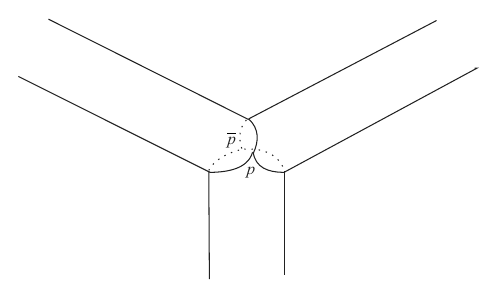
\includegraphics[width=.52\textwidth]{chapters/ch21-spectral-construction/figures/figure-21-1.png}
 \caption{一个极小面积度量。}
 \label{fig:21-minimal-area-metric}
\end{figure}

按如下方式把 $\Sigma$ 认作 $\Sigma_i$ 之并：
\[
 \Sigma=\bigcup_{i=1}^3\Sigma_i.
\]
若把 $\Sigma_i$ 等同于 $(-\infty,0]\times S^1$，则 $\Sigma$ 中存在三条从 $p$ 连接
到 $\bar p$、长度为 $1/2$ 的道路 $\theta_i$，$i=1,2,3$，使
\begin{equation}
 \begin{aligned}
 \partial_1\Sigma&=\theta_1\circ\theta_3^{-1},\\
 \partial_2\Sigma&=\theta_2\circ\theta_1^{-1},\\
 \partial_3\Sigma&=\theta_3\circ\theta_2^{-1}
 =(\theta_1\circ\theta_3^{-1})^{-1}\circ
 (\theta_2\circ\theta_1^{-1})^{-1}.
 \end{aligned}
 \label{eq:21-pants-gluing-rule}
\end{equation}
在这些坐标中，$p,\bar p$ 分别对应 $(s,t)=(0,0),(0,1/2)$。对 $i=1,2$ 固定
$\Sigma_i$ 与 $(-\infty,0]\times S^1$ 的全纯等同，其中
$S^1=\mathbb R/2\pi\mathbb Z$；并据分解~\eqref{eq:21-pants-gluing-rule} 把
$\Sigma_3$ 等同于 $[0,\infty)\times S^1$。记这些等同为
\[
 \varphi_i^-:\Sigma_i\to(-\infty,0]\times S^1,\quad i=1,2,
 \qquad
 \varphi_3^+:\Sigma_3\to[0,\infty)\times S^1,
\]
前者对应正穿孔，后者对应负穿孔；圆柱上的标准坐标记为 $(\tau,t)$。

现于三份 $[0,1]^2$ 上构造显式的哈密顿微分同胚二参数族。用
\eqref{eq:21-reparameterization-cutoff} 型函数对同痕的时间 $t$ 重参数化后，可设
$\phi_i$ 在 $t=0,1$ 附近关于时间为常值。公式为
\[
 \phi_1(s,t)=
 \begin{cases}
 \phi_{H_1}^{(1-s)t/(1-s/2)},&0\leq t\leq1-s/2,\\
 \phi_{H_1}^{1-s}\phi_{H_2}^{2(t-1+s/2)/s},&1-s/2\leq t\leq1,
 \end{cases}
\]
\[
 \phi_2(s,t)=
 \begin{cases}
 \phi_{H_1}^{2t},&0\leq t\leq s/2,\\
 \phi_{H_1}^{s}\phi_{H_2}^{(t-s/2)/(1-s/2)},&s/2\leq t\leq1,
 \end{cases}
\]
以及
\[
 \phi_3(s,t)=
 \begin{cases}
 \phi_{H_1}^{t(1+s)}\phi_{H_2}^{t(1-s)},&0\leq t\leq1-s/2,\\
 \phi_{H_1}^{(1+s)(1-s/2)}
 \phi_{H_2}^{2(t-1+s/2)/s},&1-s/2\leq t\leq1.
 \end{cases}
\]

\begin{exercise}
\label{ex:21-pants-family-compatibility}
核验该族与粘合规则~\eqref{eq:21-pants-gluing-rule} 的相容性，以及它在
$p,\bar p$ 之外的光滑性。
\end{exercise}

此外，从公式也可看出
\[
 \phi_1(0,t)=\phi_{H_1}^t,\qquad
 \phi_2(0,t)=\phi_{H_2}^t,\qquad
 \phi_3(1,t)=\phi_{H_1}^t\phi_{H_2}^t.
\]
相应联络在 $p,\bar p$ 外的平坦性，显然来自上述光滑的哈密顿微分同胚二参数族。

再用\termElongationFunction{}~$\rho$ 沿 $s$ 方向拉长裤子，得到 $\Sigma$ 上除 $p,\bar p$ 外处处光滑
的平坦联络。记平凡丛 $\dot\Sigma\times M\to\dot\Sigma$ 上的联络 1-形式为
\footnote{译者注：原文把联络 1-形式 $K$ 排成从 $\dot\Sigma$ 到
$\Omega^1(\dot\Sigma,C_0^\infty(M))$ 的映射，类型上似乎多出一层 $\dot\Sigma$；
译文照录。}
\[
 K:\dot\Sigma\longrightarrow\Omega^1(\dot\Sigma,C_0^\infty(M)).
\]
由于 $H_1,H_2$ 在边界附近平坦，它也在 $p,\bar p$ 处光滑，且曲率为 $0$。
\end{proof}

\begin{remark}
\label{rem:21-concatenation-hamiltonian}
同伦类 $[H_1\#H_2]$ 还可由拼接哈密顿量
\[
 H_1*H_2(t,x)=
 \begin{cases}
 2H_1(2t,x),&t\leq1/2,\\
 2H_2(2t-1,x),&t\geq1/2
 \end{cases}
\]
实现，而不必用 $H_1\#H_2$。这里假设 $H_1,H_2$ 在 $t=0,1$ 附近均边界平坦，
以保证相应联络光滑。这给出三元组 $(H_1,H_2;H_1*H_2)$ 所伴随的稍有不同的哈密顿
纤维化。不过 $H_1\#H_2$ 与 $H_1*H_2$ 同伦，故可把后者作为第三个哈密顿量
$H_3$；此时平坦联络的构造比使用 $H_1\#H_2$ 更明显。只须取
$\phi_3(s,t)\equiv\phi_3(0,t)$，并注意
\[
 \phi_3(0,t)=
 \begin{cases}
 \phi_{H_1}^{2t},&0\leq t\leq1/2,\\
 \phi_{H_1}^1\phi_{H_2}^{2t-1},&1/2\leq t\leq1,
 \end{cases}
\]
这正是道路 $\phi_{H_1}*\phi_{H_2}:t\mapsto\phi_{H_1*H_2}^t$。事实上，上述
$\phi_3$ 公式给出 $\phi_{H_1*H_2}$ 与 $\phi_{H_1}\phi_{H_2}$ 之间的显式同伦。
更多细节见 (FOOO11b)。
\end{remark}

现在证明三角不等式。令 $\alpha\in CF_*(H)$、$\beta\in CF_*(F)$ 是满足
$[\alpha]=a^\flat,[\beta]=b^\flat$ 的弗洛尔闭链，并令其裤子乘积闭链
$\alpha*\beta=:\gamma\in CF_*(H\#F)$。则
$[\alpha*\beta]=(a\cdot b)^\flat$，所以
\begin{equation}
 \rho(H\#F;a\cdot b)\leq\lambda_{H\#F}(\alpha*\beta).
 \label{eq:21-triangle-product-level}
\end{equation}
给定 $\delta>0$，选取 $\alpha,\beta$ 使
\begin{align}
 \lambda_H(\alpha)&\leq\rho(H;a)+\delta/2,
 \label{eq:21-alpha-near-minimax}\\
 \lambda_F(\beta)&\leq\rho(F;b)+\delta/2.
 \label{eq:21-beta-near-minimax}
\end{align}
于是可写
\[
 \alpha=\sum_i a_i[z_i,w_i],\quad
 \mathcal A_H([z_i,w_i])\leq\rho(H;a)+\delta/2,
\]
\[
 \beta=\sum_j a_j[z_j,w_j],\quad
 \mathcal A_F([z_j,w_j])\leq\rho(F;b)+\delta/2.
\]
下面用裤子乘积 (20.2.29) 估计 $\alpha*\beta\in CF_*(H\#F)$ 的层级。

回忆 (4.3.16) 与命题~\ref{prop:20-energy-curvature-identity} 中的恒等式
\[
 \int v^*\Omega_E=-\mathcal A_{H_1\#H_2}([z_3,w_3])
 +\mathcal A_{H_1}([z_1,w_1])+\mathcal A_{H_2}([z_2,w_2])
\]
及
\[
 E_{(K,J)}(u)=\int v^*\Omega_E+R_K(u),
\]
其中对任意 $u\in\mathcal M(K,J;\widetilde z)$，$v(z)=(z,u(z))$。
按 $*$ 的定义，对任意 $[z_3,w_3]\in\alpha*\beta$，存在
$[z_1,w_1]\in\alpha$、$[z_2,w_2]\in\beta$，使
$\mathcal M(K,J;\widetilde z)$ 在渐近条件
\[
 \widetilde z=([z_1,w_1],[z_2,w_2];[z_3,w_3])
\]
下非空。应用引理~\ref{lem:21-small-curvature-connection} 及
\eqref{eq:21-triangle-product-level}--\eqref{eq:21-beta-near-minimax}，立即得到
\begin{align}
 \mathcal A_{H\#F}([z_3,w_3])
 &\leq\mathcal A_H([z_1,w_1])+\mathcal A_F([z_2,w_2])+\delta\notag\\
 &\leq\lambda_H(\alpha)+\lambda_F(\beta)+\delta\notag\\
 &\leq\rho(H;a)+\rho(F;b)+2\delta
 \label{eq:21-triangle-action-estimate}
\end{align}
对所有 $[z_3,w_3]\in\alpha*\beta$ 成立。合并
\eqref{eq:21-triangle-product-level}--\eqref{eq:21-triangle-action-estimate}，有
\[
 \rho(H\#F;a\cdot b)\leq\rho(H;a)+\rho(F;b)+2\delta.
\]
令 $\delta\to0$，即得
\[
 \rho(H\#F;a\cdot b)\leq\rho(H;a)+\rho(F;b),
\]
三角不等式得证。

\section{谱性公理}
\label{sec:spectrality-axiom}

一般辛流形、特别是无理辛流形 $(M,\omega)$ 上的谱不变量 $\rho(H;a)$ 有如下最为
非平凡的性质之一：
\begin{equation}
 \text{（谱性）}\qquad \rho(H;a)\in\operatorname{Spec}(H)
 \label{eq:21-spectrality}
\end{equation}
对\emph{任意} $H$ 与 $a\in QH^*(M)$ 成立。对任意\emph{有理}辛流形，即使 $H$ 退化，这一性质
也相对容易证明；见 (Oh05c)。
\footnote{译者注：原文此处再次把谱性写成对所有 $a\in QH^*(M)$ 成立，但
定义~\ref{def:21-spectral-invariant} 只对 $a\neq0$ 定义实值谱不变量；译文照录。}

另一方面，对\emph{无理}辛流形迄今只证明了以下较弱版本；退化哈密顿量是否满足谱性仍是
未知的：
\stfhIndex{I136}{Feituihuapuxing}{非退化谱性（nondegenerate spectrality）}
\[
 \tag{非退化谱性}
 \text{对任意非退化 }H\text{ 及 }a\in QH^*(M),
 \quad\eqref{eq:21-spectrality}\text{ 成立。}
\]

\begin{question}
\label{prob:21-degenerate-irrational-spectrality}
无理辛流形上的退化哈密顿量是否满足谱性公理？若否，构造一个违反谱性公理的
哈密顿量。
\end{question}

不过，结合柔性逼近论证，这一非退化谱性足以证明一般的 $\rho(H;a)$ 同伦不变性；
\stfhIndex{I169}{JinFuluoerbilian}{紧弗洛尔闭链（tight Floer cycle）}
见 21.6 节。(Oh05c, Oh09a) 给出的谱性证明方案依赖\emph{紧弗洛尔闭链}的存在性。

\begin{definition}
\label{def:21-tight-floer-cycle}
若弗洛尔闭链 $\alpha\in CF(H)$ 满足：对任意与其同调的弗洛尔闭链
$\alpha'\in CF(H)$，即 $\alpha'-\alpha=\partial_{(H,J)}\gamma$，都有
\[
 \lambda_H(\alpha')\geq\lambda_H(\alpha),
\]
则称 $\alpha$ 是\emph{紧}的。
\end{definition}

本节尝试在起初不假设辛流形有理性的前提下证明谱性，解释这个几何论证在无理情形
下可能出错之处，再对任意哈密顿量——无论是否非退化——证明有理情形的谱性。
关于无理情形非退化谱性的完整证明，参见 (Oh09a) 或 (Ush08)。(Oh09a) 的证明是
几何的，并在称作\emph{瑟夫同伦}的通有单参数哈密顿量族下证明谱不变量的许多其他性质；
(Ush08) 的证明则是纯代数的，因为它适用于 13.8 节意义下的任意抽象弗洛尔复形。

\stfhIndex{I050}{Dianfanbozhumian}{典范薄柱面（canonical thin cylinder）}
回忆\termCanonicalThinCylinder{} (18.2.7) 的定义。重要的是，$u_{zz'}^{\mathrm{can}}$ 的像包含在
$z$（或 $z'$）的小邻域内；当 $z,z'$ 在 $C^1$ 拓扑中趋于环路 $z_\infty$ 时，它一致
收敛到 $z_\infty$。因此，在满足边界条件
\[
 u(0,t)=z(t),\qquad u(1,t)=z'(t)
\]
的映射 $u:[0,1]\times S^1\to M$ 的同伦类集合中，$u_{zz'}^{\mathrm{can}}$ 也选出
一个典范同伦类 $[u_{zz'}^{\mathrm{can}}]$。

\begin{lemma}
\label{lem:21-canonical-cylinder-area}
设 $z,z':S^1\to M$ 是两条光滑环路，$u^{\mathrm{can}}$ 是 (18.2.7) 给出的上述典范
圆柱。对 $z$ 的任意填充圆盘 $w$ 及附近环路 $z'$，关联 $z'$ 的填充圆盘
\[
 w':=w\#u_{zz'}^{\mathrm{can}}.
\]
当 $d_{C^1}(z,z')\to0$ 时，$u_{zz'}^{\mathrm{can}}$ 在 $C^1$ 拓扑中收敛，且其几何
面积 $\operatorname{Area}(u^{\mathrm{can}})$ 趋于零。特别地，当 $z'\to z$ 且
$d_{C^1}(z,z')\to0$ 时：
\footnote{译者注：原文只说 $u_{zz'}^{\mathrm{can}}$ 在 $C^1$ 拓扑中“收敛”，
却没有给出其极限；随后第 (1) 项明确陈述的是拼接圆盘 $w'\to w$。译文照录。}
\begin{enumerate}[label=(\arabic*)]
 \item 作为单位圆盘到 $M$ 的映射，$w'\to w$ 于 $C^1$ 拓扑；
 \item 辛面积满足
 \begin{equation}
  \int_{u_{zz'}^{\mathrm{can}}}\omega\longrightarrow0.
  \label{eq:21-thin-cylinder-symplectic-area}
 \end{equation}
\end{enumerate}
\end{lemma}

\begin{proof}
第 (1) 项立即来自上述\termCanonicalThinCylinder{}的显式形式及指数映射的标准性质。另一方面，由\termCanonicalThinCylinder{}的显式表达与指数映射的性质，容易作面积估计，得到当
$d_{C^1}(z,z')\to0$ 时 $\operatorname{Area}(u_{zz'}^{\mathrm{can}})\to0$。因
$z,z'$ 均为 $C^1$ 的，$u_{zz'}^{\mathrm{can}}$ 也是 $C^1$ 的，故
\[
 \operatorname{Area}(u_{zz'}^{\mathrm{can}})
 \geq\left|\int_{u_{zz'}^{\mathrm{can}}}\omega\right|.
\]
这蕴含当 $z'\to z$ 于 $C^1$ 拓扑时，
$\int_{u_{zz'}^{\mathrm{can}}}\omega\to0$。
\end{proof}

目标是证明极小极大值 $\rho(H;a)$ 是临界值，即存在
$[z,w]\in\widetilde{\mathcal L}_0(M)$ 使
\[
 \mathcal A_H([z,w])=\rho(H;a),\qquad
 d\mathcal A_H([z,w])=0,
 \quad\text{即}\quad \dot z=X_H(z).
\]
此前已证明 $\rho(H;a)$ 有限。

\begin{theorem}
\label{thm:21-rational-spectrality}
设 $(M,\omega)$ 有理，则任意哈密顿量 $H$ 均满足谱性公理，不要求 $H$ 非退化。
\end{theorem}

\begin{proof}
我们可以通过反证法证明：对于任意光滑哈密顿量，谱性公理成立，证明如下。
若 $H$ 非退化，就固定 $H$；否则在 $C^2$ 拓扑中以非退化哈密顿量序列
$H_i$ 逼近 $H$。选取弗洛尔闭链 $\alpha_i\in CF_*(H_i)$，使
$\lambda_{H_i}(\alpha_i)\to\rho(H;a)$。令
$\operatorname{peak}(\alpha_i)=[z_i,w_i]\in\operatorname{Crit}\mathcal A_{H_i}$。
则
\begin{equation}
 \lim_{i\to\infty}\mathcal A_{H_i}([z_i,w_i])=\rho(H;a).
 \label{eq:21-peak-action-limit}
\end{equation}
由 $\rho(\,\cdot\,;a)$ 的定义及有限性，可选出这样的序列。

现在我们证明序列 $[z_i,w_i]$ 在 $\widetilde{\mathcal L}_0(M)$ 上是预紧的。
因 $M$ 紧、$H_i\to H$ 于 $C^2$ 拓扑且 $\dot z_i=X_{H_i}(z_i)$，标准自举论证给出
$z_i$ 的一个子列（仍记 $z_i$）收敛到某环路 $z_\infty:S^1\to M$，且
$\dot z_\infty=X_H(z_\infty)$。由于固定了非零量子上同调类
$a\in QH^*(M)$（更具体地说，固定了它的次数），并且 $[\alpha_i]=a^\flat$，有
\[
 \mu_{H_i}([z_i,w_i])=\mu_{H_j}([z_j,w_j]).
\]

对充分大的 $i$，考虑 $z_\infty$ 的填充圆盘
\[
 w'_i=w_i\#u_{i\infty}^{\mathrm{can}},
\]
其中 $u_{i\infty}^{\mathrm{can}}=u_{z_i z_\infty}^{\mathrm{can}}$ 是 $z_i$ 与
$z_\infty$ 之间的\termCanonicalThinCylinder{}。其几何面积在 $i\to\infty$ 时趋于零。计算临界点
$[z_\infty,w'_i]\in\operatorname{Crit}\mathcal A_H$ 的作用量：
\begin{align}
 \mathcal A_H([z_\infty,w'_i])
 &=-\int_{w'_i}\omega-\int_0^1H(t,z_\infty(t))\,dt \notag\\
 &=-\int_{w_i}\omega-\int_{u_{i\infty}^{\mathrm{can}}}\omega
   -\int_0^1H(t,z_\infty(t))\,dt \notag\\
 &=\left(-\int_{w_i}\omega-\int_0^1H_i(t,z_i(t))\,dt\right)
   -\int_{u_{i\infty}^{\mathrm{can}}}\omega \notag\\
 &\quad-\left(\int_0^1H(t,z_\infty(t))\,dt
   -\int_0^1H_i(t,z_i(t))\,dt\right) \notag\\
 &=\mathcal A_{H_i}([z_i,w_i])
   -\int_{u_{i\infty}^{\mathrm{can}}}\omega \notag\\
 &\quad-\left(\int_0^1H(t,z_\infty(t))\,dt
   -\int_0^1H_i(t,z_i(t))\,dt\right).
 \label{eq:21-limit-action-computation}
\end{align}
由于 $z_i$ 一致收敛到 $z_\infty$ 且 $H_i\to H$，
\begin{equation}
 -\left(\int_0^1H(t,z_\infty(t))dt
 -\int_0^1H_i(t,z_i(t))dt\right)\longrightarrow0.
 \label{eq:21-hamiltonian-integral-limit}
\end{equation}
结合~\eqref{eq:21-peak-action-limit}--\eqref{eq:21-hamiltonian-integral-limit}，得到
\[
 \lim_{i\to\infty}\mathcal A_H([z_\infty,w'_i])=\rho(H;a).
\]
故 $\mathcal A_H([z_\infty,w'_i])$ 是柯西序列，从而
\[
 \left|\int_{w'_i}\omega-\int_{w'_j}\omega\right|
 =|\mathcal A_H([z_\infty,w'_i])-\mathcal A_H([z_\infty,w'_j])|
 \longrightarrow0,
\]
即
\[
 \int_{w'_i\#\overline{w'_j}}\omega\longrightarrow0.
\]
因 $\Gamma$ 离散且 $[w'_i\#\overline{w'_j}]_\omega\in\Gamma$，对充分大的
$i,j\in\mathbb Z_+$，必有
\begin{equation}
 \int_{w'_i\#\overline{w'_j}}\omega=0.
 \label{eq:21-rational-area-stabilization}
\end{equation}
特别地，数集 $\{\int_{w'_i}\omega\}_{i\in\mathbb Z_+}$ 有界；必要时取子列，可认为
序列 $\int_{w'_i}\omega$ 最终稳定。由 $\mathcal A_H$ 的定义，对任意充分大的 $N$，
$\mathcal A_H([z_\infty,w'_N])=
\lim_{i\to\infty}\mathcal A_H([z_\infty,w'_i])$。回到
\eqref{eq:21-limit-action-computation} 可见作用量本身稳定，故
\[
 \mathcal A_H([z_\infty,w'_N])
 =\lim_{i\to\infty}\mathcal A_H([z_\infty,w'_i])=\rho(H;a).
\]
所以 $\rho(H;a)$ 确为 $\mathcal A_H$ 在临界点 $[z_\infty,w'_N]$ 处的值。
这就是对无理情形不成立的关键所在。
\end{proof}

上述有理情形证明中，下述引理起关键作用。部分由于它在无理情形下失效，即使只论
非退化情形，无理情形谱性的证明也远比有理情形非平凡。

\begin{lemma}
\label{lem:21-rational-critical-set-compactness}
当 $(M,\omega)$ 有理时，对任意光滑哈密顿量 $K$，
$\operatorname{Crit}\mathcal A_K\subset\widetilde{\mathcal L}_0(M)$ 是
$\mathbb R$ 的闭子集，并且在覆盖空间
$\pi:\widetilde{\mathcal L}_0(M)\to\mathcal L_0(M)$ 的子空间拓扑中局部紧。
\footnote{译者注：原文称
$\operatorname{Crit}\mathcal A_K\subset\widetilde{\mathcal L}_0(M)$ 是
“$\mathbb R$ 的闭子集”，但证明只说明它在覆盖空间中闭；译文照录该类型疑点。}
\end{lemma}

\begin{proof}
当 $(M,\omega)$ 有理时，上述 $\pi$ 的覆盖群 $\Gamma$ 离散。再结合紧流形 $M$ 上
方程 $\dot z=X_K(z)$ 的解集紧，可知
\[
 \operatorname{Crit}(\mathcal A_K)
 =\{[z,w]\in\widetilde{\mathcal L}_0(M)\mid\dot z=X_K(z)\}
\]
是闭集且局部紧。
\end{proof}

无理情形非退化谱性的证明最早由 (Oh09a) 给出（半正情形）。该证明使用连续性方法，
从一个小莫尔斯函数出发沿\emph{瑟夫同伦}推进，并细致分析与谱不变量对应的临界值如何
\stfhIndex{I190}{Eshe}{厄舍（Usher）}
变化。后来厄舍 (Ush08) 基于非阿基米德分析中一条优美的逼近定理，在 13.8 节所述
弗洛尔同调公理框架中给出简洁的代数证明。这里只陈述厄舍的第 13.8 节框架下
非退化谱性公理的抽象表述；其证明
依赖紧闭链的存在性，细节见 (Ush08)。回忆定义 13.8.1 中的
$\operatorname{Spec}(\mathfrak c)$。

\begin{theorem}[定理 1.4 (Ush08)]
\label{thm:21-usher-spectrality}
设 $\mathfrak c$ 是诺特环 $R$ 上的滤过弗洛尔--诺维科夫复形。则对每个
$a\in H_*(\mathfrak c)$，存在 $\alpha\in C_*(\mathfrak c)$ 使
$[\alpha]=a$ 且 $\rho(a)=\lambda(\alpha)$。特别地，
$\rho(a)\in\operatorname{Spec}(\mathfrak c)$。
\end{theorem}

对任意非退化哈密顿量 $H$ 的弗洛尔复形
$(CF_*(H),\partial_{(H,J)})$，此定理说明谱数 $\rho(H;a)$ 由一条紧弗洛尔闭链
$\alpha$ 的层级实现，即 $\lambda_H(\alpha)=\rho(H;a)$。特别地，
$\rho(H;a)\in\operatorname{Spec}(H)$，这就证明了 $\rho(H;a)$ 的非退化谱性。

\section{同伦不变性}
\label{sec:spectral-homotopy-invariance}

下述命题说明函数 $\rho_a=\rho(\,\cdot\,;a)$ 下降为
$\widetilde{\operatorname{Ham}}(M,\omega)$ 上的连续函数。

\begin{theorem}[同伦不变性]
\label{thm:21-spectral-homotopy-invariance}
设 $(M,\omega)$ 是任意闭辛流形，并假设 $(M,\omega)$ 满足非退化谱性公理。则对任意
光滑函数 $H\sim K$，即满足 $\phi_H^1=\phi_K^1$ 且 $\phi_H,\phi_K$ 相对于端点道路
同伦的函数，都有
\begin{equation}
 \rho(\underline H;a)=\rho(\underline K;a).
 \label{eq:21-spectral-homotopy-equality}
\end{equation}
\end{theorem}

本节将给出该定理的两个不同证明，每一个都包含弗洛尔理论研究中的若干重要成分。
暂且推迟证明，先陈述其推论。由同伦不变性，可对代表
$h=[\phi_H]$ 的任意 $H$（无论 $h$ 是否非退化）定义
\begin{equation}
 \rho_a(h):=\rho(H;a).
 \label{eq:21-spectral-function-cover}
\end{equation}
这给出良定义函数
\[
 \rho_a:\widetilde{\operatorname{Ham}}(M,\omega)\longrightarrow\mathbb R.
\]

\begin{theorem}
\label{thm:21-spectral-function-continuous-cover}
在由 $P^{\mathrm{ham}}(\operatorname{Symp}(M,\omega),\mathrm{id})$ 诱导的商拓扑下，
$\rho_a$ 是 $\widetilde{\operatorname{Ham}}(M,\omega)$ 上的连续函数。
\end{theorem}

\begin{proof}
回忆商映射
\[
 \pi:P^{\mathrm{ham}}(\operatorname{Symp}(M,\omega),\mathrm{id})
 \longrightarrow\widetilde{\operatorname{Ham}}(M,\omega).
\]
已经证明赋值
\begin{equation}
 \lambda\longmapsto\rho(\lambda;a)
 \label{eq:21-spectral-function-path-space}
\end{equation}
在道路空间上连续。按商拓扑定义，
$\rho_a:\widetilde{\operatorname{Ham}}(M,\omega)\to\mathbb R$ 连续，因为复合
\[
 \rho_a\circ\pi:
 P^{\mathrm{ham}}(\operatorname{Symp}(M,\omega),\mathrm{id})\longrightarrow\mathbb R
\]
正是~\eqref{eq:21-spectral-function-path-space}。
\end{proof}

\subsection{使用非退化谱性的证明}

先考虑满足 $H\sim K$ 的非退化哈密顿量。回忆以下基本事实：
\begin{enumerate}[label=(\arabic*)]
 \item 哈密顿函数 $H$ 的非退化性只依赖其时间一映射 $\phi=\phi_H^1$；
 \item $\operatorname{Spec}(H)\subset\mathbb R$，即作用量泛函 $\mathcal A_H$ 的
 临界值集，是零测集（见 (Oh02) 的引理 2.2）；
 \item 若 $H,H'\mapsto\phi$ 且 $H\sim H'$，并且二者已归一化，则
 $\operatorname{Spec}(H)=\operatorname{Spec}(H')$（命题 18.3.6）；
 \item 函数 $H\mapsto\rho(H;a)$ 关于 $C_0^\infty(S^1\times M)$ 上的光滑拓扑连续
 （命题~\ref{prop:21-spectral-continuity}）；
 \item 从连通空间（例如区间 $[0,1]$）到 $\mathbb R$ 且值落在某个零测子集中的连续
 函数，只能是常函数。
\end{enumerate}

因 $H\sim K$，存在光滑族 $\mathcal H=\{H(s)\}_{0\leq s\leq1}$，使
$H(0)=H,H(1)=K$。定义 $\rho:[0,1]\to\mathbb R$ 为
$\rho(s)=\rho(H(s);a)$。由于所有 $s$ 的时间一映射均为
$\phi_{H(s)}^1=\phi_H^1$，$H(s)$ 都非退化；其像落在与 $s$ 无关的\emph{固定}子集
$\operatorname{Spec}(h)\subset\mathbb R$ 中，其中 $h=[H]=[K]$ 是道路同伦类。
由上述第 (2) 项，该集为零测集，因而全不连通。函数 $\rho$ 又由 $C^0$-连续性公理
连续，故必为常函数，于是
$\rho(H;a)=\rho(0)=\rho(1)=\rho(K;a)$，证明了非退化情形。
\footnote{译者注：原文此处回指第 (1) 项，但“作用谱是零测集”是上列第 (2) 项；
译文改正编号。}
\footnote{译者注：这里 $\rho$ 已被定义为参数函数 $s\mapsto\rho(H(s);a)$；原文等式
同时写 $\rho(H;a)$ 与 $\rho(0)$，记号层次混用，译文照录。}

现设 $H$ 退化。要强调的是，目前尚不知道退化哈密顿量是否满足谱性公理，因此不能
把上述非退化证明方案直接用于退化情形。改用基于下述引理的逼近论证。

\begin{lemma}
\label{lem:21-common-morse-perturbation}
设未必非退化的 $H\sim K$。则存在 $C^2$-收敛到 $0$ 的莫尔斯函数序列 $f_i$，使
$H\#f_i\sim K\#f_i$，且 $H\#f_i,K\#f_i$ 均非退化。
\end{lemma}

\begin{proof}
留作习题。
\end{proof}

应用此引理，
\[
 \rho(H;a)=\lim_{i\to\infty}\rho(H\#f_i;a)
 =\lim_{i\to\infty}\rho(K\#f_i;a)=\rho(K;a).
\]
第一种证明完成。

\stfhIndex{I147}{Zuiyouyantuo}{最优延拓（optimal continuation）}
\subsection{使用最优延拓的证明}

回忆同伦不变性的设定。给定 $H_0,H_1$，满足
$\phi_{H_0}^1=\phi_{H_1}^1$ 且 $[H_0]=[H_1]$。按定义，存在二参数族
$\{\phi(s,t)\}\subset\operatorname{Ham}(M,\omega)$，$(s,t)\in[0,1]^2$。存在
$\psi\in\operatorname{Ham}(M,\omega)$，使
\begin{equation}
 \begin{aligned}
 \phi(s,0)&\equiv\mathrm{id},&\quad \phi(s,1)&\equiv\psi
 &&\text{对所有 }s\in[0,1],\\
 \phi(0,t)&=\phi_{H_0}^t,& \phi(1,t)&=\phi_{H_1}^t
 &&\text{对所有 }t\in[0,1].
 \end{aligned}
 \label{eq:21-two-parameter-isotopy-boundary}
\end{equation}
记 $\mathcal H=H(s,t,x)$，其中 $H^s=H(s,\,\cdot\,,\,\cdot\,)$ 是生成向量场
\[
 \frac{\partial\phi}{\partial t}\circ\phi^{-1}
\]
的哈密顿量；又以 $F=F(s,t,x)$ 表示生成相应 $s$-哈密顿向量场
\[
 \frac{\partial\phi}{\partial s}\circ\phi^{-1}
\]
的哈密顿量。由~\eqref{eq:21-two-parameter-isotopy-boundary}，在 $t=0,1$ 附近沿
$t$ 方向、在 $s=0,1$ 附近沿 $s$ 方向重参数化
$\phi:[0,1]^2\to\operatorname{Ham}(M,\omega)$ 后，可设
\[
 F\equiv0\quad\text{于}\quad
 ([0,\epsilon]\times[0,1])\cup([1-\epsilon,1]\times[0,1]),
\]
特别地，$s$-哈密顿向量场 $X_F$ 对每个 $s$ 都关于 $t$ 一周期。

对给定 $[z^-,w^-]$、$[z^+,w^+]$，且
$[w^-\#u]=[w^+]\in\pi_2(z^+)$，考虑扰动柯西--黎曼方程
\begin{equation}
 \begin{cases}
 \partial u/\partial\tau-X_{F^\rho}(u)
 +J(\partial u/\partial t-X_{H^\rho}(u))=0,\\
 u(-\infty)=z^-,\quad u(\infty)=z^+,
 \end{cases}
 \label{eq:21-optimal-continuation-equation}
\end{equation}
并寻找有限能量解，其中
\[
 E_{(\phi^\rho,J)}(u):=\frac12\int_{\mathbb R\times[0,1]}
 \left(
 \left\lVert\frac{\partial u}{\partial\tau}-X_{F^\rho}(u)\right\rVert_J^2
 +\left\lVert\frac{\partial u}{\partial t}-X_{H^\rho}(u)\right\rVert_J^2
 \right).
\]
此方程等价于 $(du+P_{(K,J)}(u))^{0,1}=0$，其中
$K=H^\rho dt+F^\rho d\tau$。由于 $(H,F)$ 来自二参数族 $\phi$，有 $R_K\equiv0$。
又因 $F$ 在 $s=0,1$ 附近为 $0$，对充分大的 $R>0$，当 $|\tau|>R$ 时
$F^\rho\equiv0$。特别地，$\tau<-R$ 时~\eqref{eq:21-optimal-continuation-equation}
成为
\[
 \frac{\partial u}{\partial\tau}
 +J\left(\frac{\partial u}{\partial t}-X_{H_0}(u)\right)=0,
\]
而 $\tau>R$ 时成为
\[
 \frac{\partial u}{\partial\tau}
 +J\left(\frac{\partial u}{\partial t}-X_{H_1}(u)\right)=0.
\]

考察零维模空间以定义映射
\[
 h_{(\phi^\rho,J)}:CF(H_0,J_0)\longrightarrow CF(H_1,J_1),
\]
再如前考察一维模空间以证明它是链映射。还要分析该链映射如何影响弗洛尔复形的
滤过；为此，\emph{当}~\eqref{eq:21-optimal-continuation-equation} 有\emph{有限}能量解时，需研究
作用量差
\[
 \mathcal A_{H_0}([z^-,w^-])-
 \mathcal A_{H_1}([z^+,w^-\#u]).
\]
先回忆基本恒等式
\begin{equation}
 R_K=\frac{\partial F^\rho}{\partial t}
 -\frac{\partial H^\rho}{\partial\tau}
 +\{F^\rho,H^\rho\}=0.
 \label{eq:21-flat-curvature-identity}
\end{equation}
这是因为对子 $(H^\rho,F^\rho)$ 来自二参数同痕
$\phi=\phi(s,t)\in\operatorname{Ham}(M,\omega)$。对
\eqref{eq:21-optimal-continuation-equation} 应用命题
\ref{prop:20-energy-curvature-identity}，并用 $R_K=0$，得到
\[
 \mathcal A_{H_1}([z^+,w^-\#u])-\mathcal A_{H_0}([z^-,w^-])
 =-E_{(\phi^\rho,J)}(u)\leq0.
\]

\begin{proposition}
\label{prop:21-optimal-continuation-action}
设 $\phi=\{\phi(s,t)\}$ 及其相应对子 $(H,F)$ 如上。令
$\rho:\mathbb R\to[0,1]$ 光滑，且对某个 $R>0$，在 $\tau\leq-R$ 时
$\rho\equiv0$，在 $\tau\geq R$ 时 $\rho\equiv1$。给定
$[z^-,w^-]\in\operatorname{Crit}\mathcal A_{H_0}$，设
$u:\mathbb R\times[0,1]\to M$ 是~\eqref{eq:21-optimal-continuation-equation} 的解，
满足 $u(-\infty)=z^-,u(\infty)=z^+$。则
\begin{equation}
 \mathcal A_{H_1}([z^+,w^-\#u])
 \leq\mathcal A_{H_0}([z^-,w^-]).
 \label{eq:21-optimal-continuation-action-bound}
\end{equation}
\end{proposition}

立即得到：

\begin{corollary}
\label{cor:21-optimal-continuation-filtration}
链映射 $h_{(\phi;J)}:CF(H_0,J_0)\to CF(H_1,J_1)$ 保持滤过，即对所有
$\lambda\in\mathbb R$ 诱导链映射
\[
 h_{(\phi;J)}^\lambda:CF^\lambda(H_0,J_0)
 \longrightarrow CF^\lambda(H_1,J_1).
\]
\end{corollary}

显然，$s$-时间反演同痕
\[
 \widetilde\phi(s,t):=\phi(1-s,t)
\]
诱导保滤过映射
$h_{(\widetilde\phi;\widetilde J)}:
CF^\lambda(H_1,J_1)\to CF^\lambda(H_0,J_0)$。

现在完成 $\rho(H_0;a)=\rho(H_1;a)$ 的证明。只须证
$\rho(H_0;a)\leq\rho(H_1;a)$，反向同理，只需考虑 $s$-时间反演。给定
$\epsilon>0$，存在弗洛尔链 $\alpha_{H_1}$，使
$[\alpha_{H_1}]=a^\flat$ 且
$\lambda_{H_1}(\alpha_{H_1})\leq\rho(H_1;a)+\epsilon$。于是
\[
 \lambda_{H_0}\bigl(h_{(\widetilde\phi;\widetilde J)}(\alpha_{H_1})\bigr)
 \leq\lambda_{H_1}(\alpha_{H_1})\leq\rho(H_1;a)+\epsilon.
\]
又因 $h_{(\widetilde\phi;\widetilde J)}(\alpha_{H_1})\in CF_*(H_0)$ 且其同调类为
$a^\flat$，
\[
 \rho(H_0;a)
 \leq\lambda_{H_0}\bigl(h_{(\widetilde\phi;\widetilde J)}(\alpha_{H_1})\bigr)
 \leq\rho(H_1;a)+\epsilon.
\]
令 $\epsilon\to0$ 即得 $\rho(H_0;a)\leq\rho(H_1;a)$。这证明了哈密顿微分同胚
$\psi=\phi_{H_0}^1=\phi_{H_1}^1$ 非退化时的结论。一般情形由
$H\mapsto\rho(H;a)$ 的 $C^0$-连续性推出。

